\section{Durchführung}
\label{sec:Durchführung}
Für die Durchführung dieses Versuches werden lediglich ein Geiger-Müller-Zählrohr, im folgendem durch \textit{GMZ} abgekürzt, und $\beta$\,-Strahler benötigt. Der Aufbau der
verwendeten Messapparatur wird in \autoref{fig:GMZ-Skizze} dargestellt. Die Funktionsweise und der Aufbau des \textit{GMZ's} wurden bereits im \autoref{sec:Theorie} diskutiert.

\begin{figure}
    \centering
    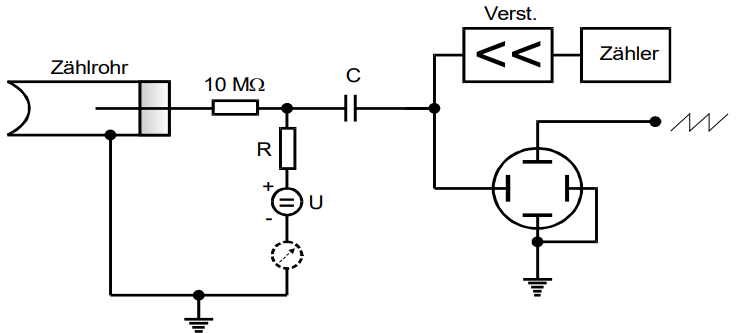
\includegraphics[width = .8\textwidth]{content/Messapparatur.PNG}
    \caption{In dieser Abbildung ist der Aufbau der verwendeten Messapparatur skizziert. \cite{v703}}
    \label{fig:GMZ-Skizze}
\end{figure}

Zunächst wird nun die Charakteristik des Zählrohes aufgenommen. Dazu wird ein $\beta$\,-Strahler vor dem Zählrohr platziert. Das Zählrohr wird nun bei unterschiedlichen
Spannungen betrieben. Dabei wird ein Spannungsintervall von $\qty{320}{\volt}$ bis $\qty{700}{\volt}$ durchlaufen, wobei das Messzeitintervall groß genug gewählt werden muss, damit
der statistische Fehler jedes Messpunktes klein ist. Bei der verwendeten Messapparatur wird dafür $\qty{120}{\second}$ bei jeder Spannung gemessen. 

Daraufhin wird die \textit{Nachentladung} untersucht. Dazu wird das Zählrohr an ein \textit{Oszilloskop} angeschlossen. Dann wird die Strahlungsintensität des 
$\beta$\,-Strahlers abgesenkt. Dazu ist eine Ablenkgeschwindigkeit von circa $\qty{50}{\micro\second\per\centi\metre}$ ausreichend. Dann wird die Spannung zunächst auf circa
$\qty{350}{\volt}$ gesenkt, sodass die Nachentladung vernachlässigbar wird. Ist die Apparatur korrekt eingestellt wird die Spannung auf $\qty{700}{\volt}$ gestellt. Das 
resultierende Bild des Oszilloskops kann dann ausgewertet werden. 

Zuletzt wird über die \textit{Zwei-Quellen-Methode} die Totzeit des Zählrohrs bestimmt. Dazu werden zunächst zwei unterschiedliche $\beta$\,-Strahler mit dem Zählrohr 
abgemessen. Dann werden beiden Stahler gleichzeitig vermessen. Dies geschieht bei einer Spannung von $\qty{500}{\volt}$. Dabei wird bei jeder Messung erneut der statistische
Fehler klein gehalten. Diese drei Messungen genügen, damit die Totzeit über den Quotienten
\begin{equation}
    \label{eqn:2_Quellen}
    T \approx \frac{N_1 + N_2 - N_{12}}{2N_1 N_2}
\end{equation}
genähert werden kann. Die Ausdrücke $N_i$ sind die Zählraten des \textit{GMZ} der $i$-ten Quelle.
